\documentclass[10pt]{article}
\usepackage[T1]{fontenc}
\usepackage{lmodern}
\usepackage{mathtools}
\usepackage{booktabs}
\usepackage{adjustbox}
\usepackage[left=1.5cm, right=2cm, top=1.5cm, bottom=2cm]{geometry}
\usepackage{tikz}
\usepackage{pgfplots}
\pgfplotsset{compat=1.18}
\usetikzlibrary{arrows.meta,positioning,calc}
\setlength\parindent{0pt}
\title{g7 1 - No Protection - Custom Algorithm - Descending}
\date{}
\author{}

\begin{document}
\maketitle
\section*{Topology}
\begin{center}\begin{adjustbox}{max width=\linewidth}
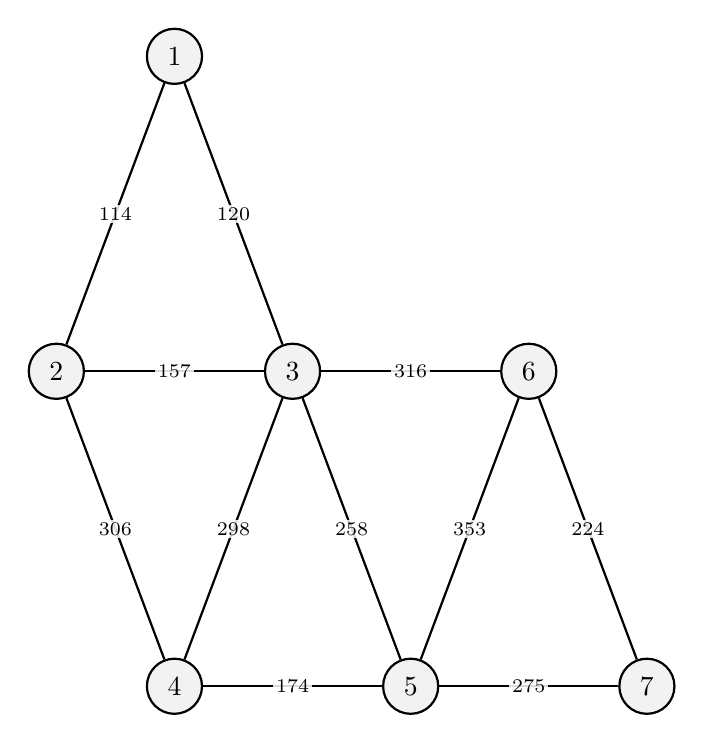
\begin{tikzpicture}[baseline, >={Stealth[length=2mm]},
  netnode/.style={circle, draw, thick, fill=gray!10, minimum size=7mm, inner sep=1pt},
  link/.style={thick},
  linklabel/.style={font=\scriptsize, inner sep=1pt, fill=white, fill opacity=0.85, text opacity=1}]
\node[netnode] (S1) at (1.500,8.000) {1};
\node[netnode] (S2) at (0.000,4.000) {2};
\node[netnode] (S3) at (3.000,4.000) {3};
\node[netnode] (S4) at (1.500,0.000) {4};
\node[netnode] (S5) at (4.500,0.000) {5};
\node[netnode] (S6) at (6.000,4.000) {6};
\node[netnode] (S7) at (7.500,0.000) {7};
\draw[link] (S1) to node[linklabel] {114} (S2);
\draw[link] (S1) to node[linklabel] {120} (S3);
\draw[link] (S2) to node[linklabel] {157} (S3);
\draw[link] (S2) to node[linklabel] {306} (S4);
\draw[link] (S3) to node[linklabel] {298} (S4);
\draw[link] (S3) to node[linklabel] {258} (S5);
\draw[link] (S3) to node[linklabel] {316} (S6);
\draw[link] (S4) to node[linklabel] {174} (S5);
\draw[link] (S5) to node[linklabel] {353} (S6);
\draw[link] (S5) to node[linklabel] {275} (S7);
\draw[link] (S6) to node[linklabel] {224} (S7);
\end{tikzpicture}
\end{adjustbox}\end{center}
\section*{Performance Parameters}
\begin{center}\begin{tabular}{lr}
\toprule
Highest link load & 73 Gb/s \\
Highest used FSU & 120 / 320 \\
Total used FSUs & 117 \\
Transponder cost & 58.5 \\
\midrule
SC-DP-QPSK transponders & 39 \\
SC-DP-16QAM transponders & 0 \\
DP-16QAM transponders & 0 \\
\bottomrule
\end{tabular}\end{center}
\clearpage
\section*{Link Load Map}
\begin{center}\begin{adjustbox}{max width=\linewidth}
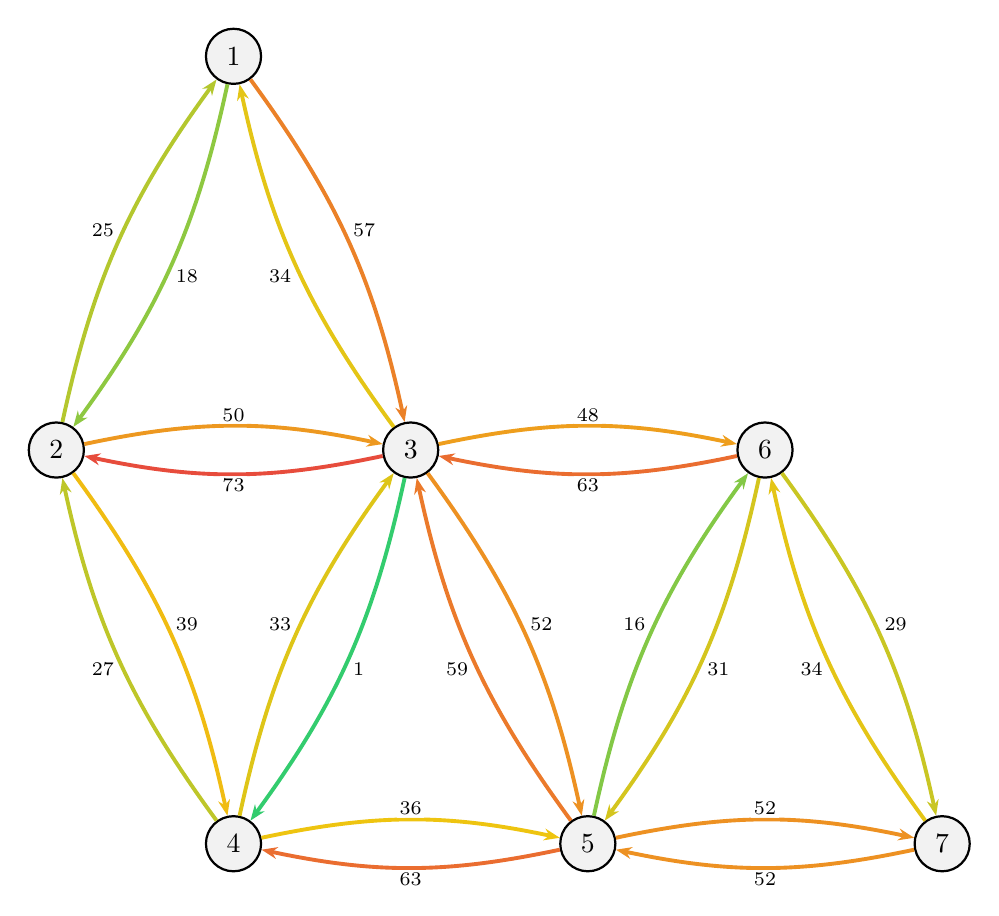
\begin{tikzpicture}[baseline, >={Stealth[length=2mm]},
  netnode/.style={circle, draw, thick, fill=gray!10, minimum size=7mm, inner sep=1pt},
  link/.style={line width=1.4pt},
  linklabel/.style={font=\scriptsize, inner sep=1pt, fill=white, fill opacity=0.85, text opacity=1}]
\node[netnode] (S1) at (2.250,10.000) {1};
\node[netnode] (S2) at (0.000,5.000) {2};
\node[netnode] (S3) at (4.500,5.000) {3};
\node[netnode] (S4) at (2.250,0.000) {4};
\node[netnode] (S5) at (6.750,0.000) {5};
\node[netnode] (S6) at (9.000,5.000) {6};
\node[netnode] (S7) at (11.250,0.000) {7};
\draw[link, ->, draw={rgb,255:red,142;green,200;blue,65}] (S1) to[bend left=12] node[linklabel, auto] {18} (S2);
\draw[link, ->, draw={rgb,255:red,235;green,129;blue,40}] (S1) to[bend left=12] node[linklabel, auto] {57} (S3);
\draw[link, ->, draw={rgb,255:red,180;green,199;blue,46}] (S2) to[bend left=12] node[linklabel, auto] {25} (S1);
\draw[link, ->, draw={rgb,255:red,237;green,152;blue,32}] (S2) to[bend left=12] node[linklabel, auto] {50} (S3);
\draw[link, ->, draw={rgb,255:red,240;green,188;blue,18}] (S2) to[bend left=12] node[linklabel, auto] {39} (S4);
\draw[link, ->, draw={rgb,255:red,228;green,197;blue,22}] (S3) to[bend left=12] node[linklabel, auto] {34} (S1);
\draw[link, ->, draw={rgb,255:red,231;green,76;blue,60}] (S3) to[bend left=12] node[linklabel, auto] {73} (S2);
\draw[link, ->, draw={rgb,255:red,51;green,204;blue,110}] (S3) to[bend left=12] node[linklabel, auto] {1} (S4);
\draw[link, ->, draw={rgb,255:red,237;green,145;blue,34}] (S3) to[bend left=12] node[linklabel, auto] {52} (S5);
\draw[link, ->, draw={rgb,255:red,238;green,158;blue,29}] (S3) to[bend left=12] node[linklabel, auto] {48} (S6);
\draw[link, ->, draw={rgb,255:red,190;green,198;blue,41}] (S4) to[bend left=12] node[linklabel, auto] {27} (S2);
\draw[link, ->, draw={rgb,255:red,222;green,197;blue,24}] (S4) to[bend left=12] node[linklabel, auto] {33} (S3);
\draw[link, ->, draw={rgb,255:red,238;green,196;blue,16}] (S4) to[bend left=12] node[linklabel, auto] {36} (S5);
\draw[link, ->, draw={rgb,255:red,235;green,122;blue,43}] (S5) to[bend left=12] node[linklabel, auto] {59} (S3);
\draw[link, ->, draw={rgb,255:red,234;green,109;blue,48}] (S5) to[bend left=12] node[linklabel, auto] {63} (S4);
\draw[link, ->, draw={rgb,255:red,131;green,200;blue,70}] (S5) to[bend left=12] node[linklabel, auto] {16} (S6);
\draw[link, ->, draw={rgb,255:red,237;green,145;blue,34}] (S5) to[bend left=12] node[linklabel, auto] {52} (S7);
\draw[link, ->, draw={rgb,255:red,234;green,109;blue,48}] (S6) to[bend left=12] node[linklabel, auto] {63} (S3);
\draw[link, ->, draw={rgb,255:red,212;green,197;blue,30}] (S6) to[bend left=12] node[linklabel, auto] {31} (S5);
\draw[link, ->, draw={rgb,255:red,201;green,198;blue,35}] (S6) to[bend left=12] node[linklabel, auto] {29} (S7);
\draw[link, ->, draw={rgb,255:red,237;green,145;blue,34}] (S7) to[bend left=12] node[linklabel, auto] {52} (S5);
\draw[link, ->, draw={rgb,255:red,228;green,197;blue,22}] (S7) to[bend left=12] node[linklabel, auto] {34} (S6);
\end{tikzpicture}
\end{adjustbox}\end{center}
\begin{center}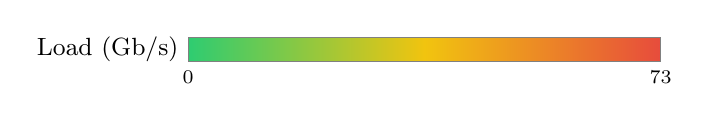
\begin{tikzpicture}
\definecolor{scalelow}{RGB}{46,204,113}\definecolor{scalemid}{RGB}{241,196,15}\definecolor{scalehigh}{RGB}{231,76,60}
\shade[left color=scalelow, right color=scalemid] (0,0) rectangle (3,0.3);
\shade[left color=scalemid, right color=scalehigh] (3,0) rectangle (6,0.3);
\draw[gray] (0,0) rectangle (6,0.3);
\node[below, font=\scriptsize] at (0,0) {0};
\node[below, font=\scriptsize] at (6,0) {73};
\node[left, font=\small] at (0,0.15) {Load (Gb/s)};
\end{tikzpicture}\end{center}
\section*{Link Load Distribution}

\begin{center}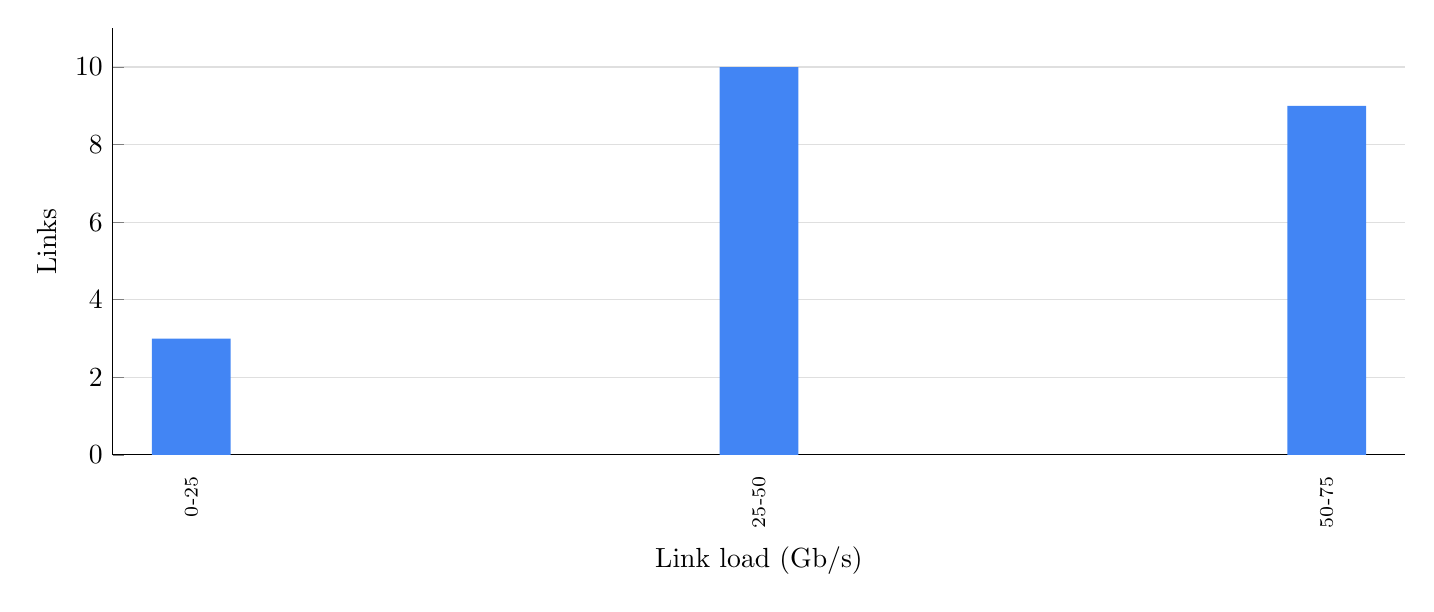
\begin{tikzpicture}
\begin{axis}[
  ybar, bar width=1.000cm, width=18.000cm, height=7cm,
  ymin=0, ymajorgrids, grid style={gray!25}, axis lines*=left,
  enlarge x limits={abs=1.000cm}, xtick=data, major x tick style={draw=none},
  x tick label style={rotate=90, font=\scriptsize, /pgf/number format/1000 sep=},
  legend style={at={(0.5,-0.3)}, anchor=north, legend columns=-1, draw=none},
  ylabel={Links},
  xlabel={Link load (Gb/s)},
  symbolic x coords={0-25,25-50,50-75}]
\addplot[fill={rgb,255:red,66;green,133;blue,244}, draw=none] coordinates {(0-25,3.000) (25-50,10.000) (50-75,9.000) };
\end{axis}
\end{tikzpicture}\end{center}
\clearpage
\section*{Spectrum Occupancy}
\begin{center}\begin{adjustbox}{max width=\linewidth}
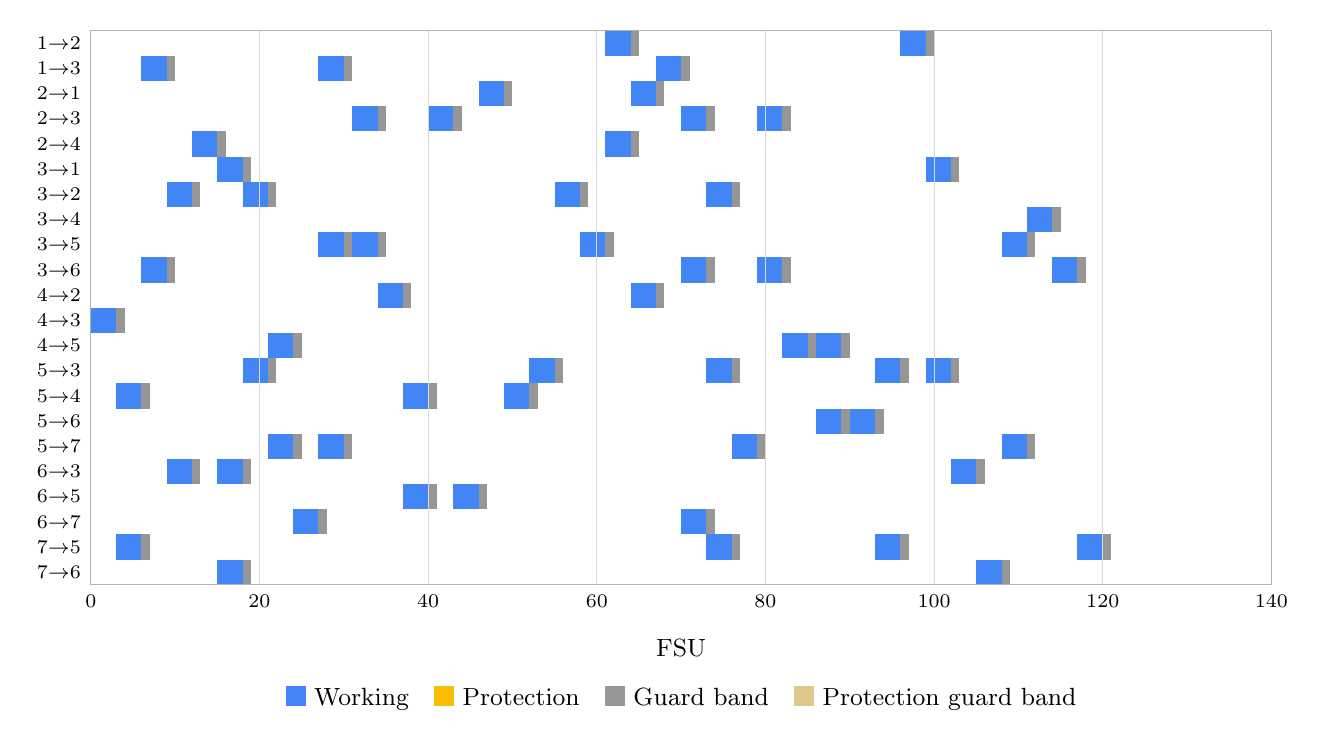
\begin{tikzpicture}[x=0.1071cm, y=-0.32cm]
\fill[fill={rgb,255:red,66;green,133;blue,244}] (61,0) rectangle (64,1);
\fill[fill={rgb,255:red,150;green,150;blue,150}] (64,0) rectangle (65,1);
\fill[fill={rgb,255:red,66;green,133;blue,244}] (96,0) rectangle (99,1);
\fill[fill={rgb,255:red,150;green,150;blue,150}] (99,0) rectangle (100,1);
\node[left, font=\scriptsize] at (0,0.5) {1\(\to\)2};
\fill[fill={rgb,255:red,66;green,133;blue,244}] (6,1) rectangle (9,2);
\fill[fill={rgb,255:red,150;green,150;blue,150}] (9,1) rectangle (10,2);
\fill[fill={rgb,255:red,66;green,133;blue,244}] (27,1) rectangle (30,2);
\fill[fill={rgb,255:red,150;green,150;blue,150}] (30,1) rectangle (31,2);
\fill[fill={rgb,255:red,66;green,133;blue,244}] (67,1) rectangle (70,2);
\fill[fill={rgb,255:red,150;green,150;blue,150}] (70,1) rectangle (71,2);
\node[left, font=\scriptsize] at (0,1.5) {1\(\to\)3};
\fill[fill={rgb,255:red,66;green,133;blue,244}] (46,2) rectangle (49,3);
\fill[fill={rgb,255:red,150;green,150;blue,150}] (49,2) rectangle (50,3);
\fill[fill={rgb,255:red,66;green,133;blue,244}] (64,2) rectangle (67,3);
\fill[fill={rgb,255:red,150;green,150;blue,150}] (67,2) rectangle (68,3);
\node[left, font=\scriptsize] at (0,2.5) {2\(\to\)1};
\fill[fill={rgb,255:red,66;green,133;blue,244}] (31,3) rectangle (34,4);
\fill[fill={rgb,255:red,150;green,150;blue,150}] (34,3) rectangle (35,4);
\fill[fill={rgb,255:red,66;green,133;blue,244}] (40,3) rectangle (43,4);
\fill[fill={rgb,255:red,150;green,150;blue,150}] (43,3) rectangle (44,4);
\fill[fill={rgb,255:red,66;green,133;blue,244}] (70,3) rectangle (73,4);
\fill[fill={rgb,255:red,150;green,150;blue,150}] (73,3) rectangle (74,4);
\fill[fill={rgb,255:red,66;green,133;blue,244}] (79,3) rectangle (82,4);
\fill[fill={rgb,255:red,150;green,150;blue,150}] (82,3) rectangle (83,4);
\node[left, font=\scriptsize] at (0,3.5) {2\(\to\)3};
\fill[fill={rgb,255:red,66;green,133;blue,244}] (12,4) rectangle (15,5);
\fill[fill={rgb,255:red,150;green,150;blue,150}] (15,4) rectangle (16,5);
\fill[fill={rgb,255:red,66;green,133;blue,244}] (61,4) rectangle (64,5);
\fill[fill={rgb,255:red,150;green,150;blue,150}] (64,4) rectangle (65,5);
\node[left, font=\scriptsize] at (0,4.5) {2\(\to\)4};
\fill[fill={rgb,255:red,66;green,133;blue,244}] (15,5) rectangle (18,6);
\fill[fill={rgb,255:red,150;green,150;blue,150}] (18,5) rectangle (19,6);
\fill[fill={rgb,255:red,66;green,133;blue,244}] (99,5) rectangle (102,6);
\fill[fill={rgb,255:red,150;green,150;blue,150}] (102,5) rectangle (103,6);
\node[left, font=\scriptsize] at (0,5.5) {3\(\to\)1};
\fill[fill={rgb,255:red,66;green,133;blue,244}] (9,6) rectangle (12,7);
\fill[fill={rgb,255:red,150;green,150;blue,150}] (12,6) rectangle (13,7);
\fill[fill={rgb,255:red,66;green,133;blue,244}] (18,6) rectangle (21,7);
\fill[fill={rgb,255:red,150;green,150;blue,150}] (21,6) rectangle (22,7);
\fill[fill={rgb,255:red,66;green,133;blue,244}] (55,6) rectangle (58,7);
\fill[fill={rgb,255:red,150;green,150;blue,150}] (58,6) rectangle (59,7);
\fill[fill={rgb,255:red,66;green,133;blue,244}] (73,6) rectangle (76,7);
\fill[fill={rgb,255:red,150;green,150;blue,150}] (76,6) rectangle (77,7);
\node[left, font=\scriptsize] at (0,6.5) {3\(\to\)2};
\fill[fill={rgb,255:red,66;green,133;blue,244}] (111,7) rectangle (114,8);
\fill[fill={rgb,255:red,150;green,150;blue,150}] (114,7) rectangle (115,8);
\node[left, font=\scriptsize] at (0,7.5) {3\(\to\)4};
\fill[fill={rgb,255:red,66;green,133;blue,244}] (27,8) rectangle (30,9);
\fill[fill={rgb,255:red,150;green,150;blue,150}] (30,8) rectangle (31,9);
\fill[fill={rgb,255:red,66;green,133;blue,244}] (31,8) rectangle (34,9);
\fill[fill={rgb,255:red,150;green,150;blue,150}] (34,8) rectangle (35,9);
\fill[fill={rgb,255:red,66;green,133;blue,244}] (58,8) rectangle (61,9);
\fill[fill={rgb,255:red,150;green,150;blue,150}] (61,8) rectangle (62,9);
\fill[fill={rgb,255:red,66;green,133;blue,244}] (108,8) rectangle (111,9);
\fill[fill={rgb,255:red,150;green,150;blue,150}] (111,8) rectangle (112,9);
\node[left, font=\scriptsize] at (0,8.5) {3\(\to\)5};
\fill[fill={rgb,255:red,66;green,133;blue,244}] (6,9) rectangle (9,10);
\fill[fill={rgb,255:red,150;green,150;blue,150}] (9,9) rectangle (10,10);
\fill[fill={rgb,255:red,66;green,133;blue,244}] (70,9) rectangle (73,10);
\fill[fill={rgb,255:red,150;green,150;blue,150}] (73,9) rectangle (74,10);
\fill[fill={rgb,255:red,66;green,133;blue,244}] (79,9) rectangle (82,10);
\fill[fill={rgb,255:red,150;green,150;blue,150}] (82,9) rectangle (83,10);
\fill[fill={rgb,255:red,66;green,133;blue,244}] (114,9) rectangle (117,10);
\fill[fill={rgb,255:red,150;green,150;blue,150}] (117,9) rectangle (118,10);
\node[left, font=\scriptsize] at (0,9.5) {3\(\to\)6};
\fill[fill={rgb,255:red,66;green,133;blue,244}] (34,10) rectangle (37,11);
\fill[fill={rgb,255:red,150;green,150;blue,150}] (37,10) rectangle (38,11);
\fill[fill={rgb,255:red,66;green,133;blue,244}] (64,10) rectangle (67,11);
\fill[fill={rgb,255:red,150;green,150;blue,150}] (67,10) rectangle (68,11);
\node[left, font=\scriptsize] at (0,10.5) {4\(\to\)2};
\fill[fill={rgb,255:red,66;green,133;blue,244}] (0,11) rectangle (3,12);
\fill[fill={rgb,255:red,150;green,150;blue,150}] (3,11) rectangle (4,12);
\node[left, font=\scriptsize] at (0,11.5) {4\(\to\)3};
\fill[fill={rgb,255:red,66;green,133;blue,244}] (21,12) rectangle (24,13);
\fill[fill={rgb,255:red,150;green,150;blue,150}] (24,12) rectangle (25,13);
\fill[fill={rgb,255:red,66;green,133;blue,244}] (82,12) rectangle (85,13);
\fill[fill={rgb,255:red,150;green,150;blue,150}] (85,12) rectangle (86,13);
\fill[fill={rgb,255:red,66;green,133;blue,244}] (86,12) rectangle (89,13);
\fill[fill={rgb,255:red,150;green,150;blue,150}] (89,12) rectangle (90,13);
\node[left, font=\scriptsize] at (0,12.5) {4\(\to\)5};
\fill[fill={rgb,255:red,66;green,133;blue,244}] (18,13) rectangle (21,14);
\fill[fill={rgb,255:red,150;green,150;blue,150}] (21,13) rectangle (22,14);
\fill[fill={rgb,255:red,66;green,133;blue,244}] (52,13) rectangle (55,14);
\fill[fill={rgb,255:red,150;green,150;blue,150}] (55,13) rectangle (56,14);
\fill[fill={rgb,255:red,66;green,133;blue,244}] (73,13) rectangle (76,14);
\fill[fill={rgb,255:red,150;green,150;blue,150}] (76,13) rectangle (77,14);
\fill[fill={rgb,255:red,66;green,133;blue,244}] (93,13) rectangle (96,14);
\fill[fill={rgb,255:red,150;green,150;blue,150}] (96,13) rectangle (97,14);
\fill[fill={rgb,255:red,66;green,133;blue,244}] (99,13) rectangle (102,14);
\fill[fill={rgb,255:red,150;green,150;blue,150}] (102,13) rectangle (103,14);
\node[left, font=\scriptsize] at (0,13.5) {5\(\to\)3};
\fill[fill={rgb,255:red,66;green,133;blue,244}] (3,14) rectangle (6,15);
\fill[fill={rgb,255:red,150;green,150;blue,150}] (6,14) rectangle (7,15);
\fill[fill={rgb,255:red,66;green,133;blue,244}] (37,14) rectangle (40,15);
\fill[fill={rgb,255:red,150;green,150;blue,150}] (40,14) rectangle (41,15);
\fill[fill={rgb,255:red,66;green,133;blue,244}] (49,14) rectangle (52,15);
\fill[fill={rgb,255:red,150;green,150;blue,150}] (52,14) rectangle (53,15);
\node[left, font=\scriptsize] at (0,14.5) {5\(\to\)4};
\fill[fill={rgb,255:red,66;green,133;blue,244}] (86,15) rectangle (89,16);
\fill[fill={rgb,255:red,150;green,150;blue,150}] (89,15) rectangle (90,16);
\fill[fill={rgb,255:red,66;green,133;blue,244}] (90,15) rectangle (93,16);
\fill[fill={rgb,255:red,150;green,150;blue,150}] (93,15) rectangle (94,16);
\node[left, font=\scriptsize] at (0,15.5) {5\(\to\)6};
\fill[fill={rgb,255:red,66;green,133;blue,244}] (21,16) rectangle (24,17);
\fill[fill={rgb,255:red,150;green,150;blue,150}] (24,16) rectangle (25,17);
\fill[fill={rgb,255:red,66;green,133;blue,244}] (27,16) rectangle (30,17);
\fill[fill={rgb,255:red,150;green,150;blue,150}] (30,16) rectangle (31,17);
\fill[fill={rgb,255:red,66;green,133;blue,244}] (76,16) rectangle (79,17);
\fill[fill={rgb,255:red,150;green,150;blue,150}] (79,16) rectangle (80,17);
\fill[fill={rgb,255:red,66;green,133;blue,244}] (108,16) rectangle (111,17);
\fill[fill={rgb,255:red,150;green,150;blue,150}] (111,16) rectangle (112,17);
\node[left, font=\scriptsize] at (0,16.5) {5\(\to\)7};
\fill[fill={rgb,255:red,66;green,133;blue,244}] (9,17) rectangle (12,18);
\fill[fill={rgb,255:red,150;green,150;blue,150}] (12,17) rectangle (13,18);
\fill[fill={rgb,255:red,66;green,133;blue,244}] (15,17) rectangle (18,18);
\fill[fill={rgb,255:red,150;green,150;blue,150}] (18,17) rectangle (19,18);
\fill[fill={rgb,255:red,66;green,133;blue,244}] (102,17) rectangle (105,18);
\fill[fill={rgb,255:red,150;green,150;blue,150}] (105,17) rectangle (106,18);
\node[left, font=\scriptsize] at (0,17.5) {6\(\to\)3};
\fill[fill={rgb,255:red,66;green,133;blue,244}] (37,18) rectangle (40,19);
\fill[fill={rgb,255:red,150;green,150;blue,150}] (40,18) rectangle (41,19);
\fill[fill={rgb,255:red,66;green,133;blue,244}] (43,18) rectangle (46,19);
\fill[fill={rgb,255:red,150;green,150;blue,150}] (46,18) rectangle (47,19);
\node[left, font=\scriptsize] at (0,18.5) {6\(\to\)5};
\fill[fill={rgb,255:red,66;green,133;blue,244}] (24,19) rectangle (27,20);
\fill[fill={rgb,255:red,150;green,150;blue,150}] (27,19) rectangle (28,20);
\fill[fill={rgb,255:red,66;green,133;blue,244}] (70,19) rectangle (73,20);
\fill[fill={rgb,255:red,150;green,150;blue,150}] (73,19) rectangle (74,20);
\node[left, font=\scriptsize] at (0,19.5) {6\(\to\)7};
\fill[fill={rgb,255:red,66;green,133;blue,244}] (3,20) rectangle (6,21);
\fill[fill={rgb,255:red,150;green,150;blue,150}] (6,20) rectangle (7,21);
\fill[fill={rgb,255:red,66;green,133;blue,244}] (73,20) rectangle (76,21);
\fill[fill={rgb,255:red,150;green,150;blue,150}] (76,20) rectangle (77,21);
\fill[fill={rgb,255:red,66;green,133;blue,244}] (93,20) rectangle (96,21);
\fill[fill={rgb,255:red,150;green,150;blue,150}] (96,20) rectangle (97,21);
\fill[fill={rgb,255:red,66;green,133;blue,244}] (117,20) rectangle (120,21);
\fill[fill={rgb,255:red,150;green,150;blue,150}] (120,20) rectangle (121,21);
\node[left, font=\scriptsize] at (0,20.5) {7\(\to\)5};
\fill[fill={rgb,255:red,66;green,133;blue,244}] (15,21) rectangle (18,22);
\fill[fill={rgb,255:red,150;green,150;blue,150}] (18,21) rectangle (19,22);
\fill[fill={rgb,255:red,66;green,133;blue,244}] (105,21) rectangle (108,22);
\fill[fill={rgb,255:red,150;green,150;blue,150}] (108,21) rectangle (109,22);
\node[left, font=\scriptsize] at (0,21.5) {7\(\to\)6};
\foreach \s in {0,20,...,140} {\draw[gray!30] (\s,0) -- (\s,22); \node[below, font=\scriptsize] at (\s,22) {\s};}
\draw[gray!60] (0,0) rectangle (140,22);
\node[font=\small] at (70.0,24.5) {FSU};
\node[font=\small] at (70.0,26.5) {\textcolor[RGB]{66,133,244}{\rule{2.5mm}{2.5mm}} Working\quad \textcolor[RGB]{251,188,5}{\rule{2.5mm}{2.5mm}} Protection\quad \textcolor[RGB]{150,150,150}{\rule{2.5mm}{2.5mm}} Guard band\quad \textcolor[RGB]{222,200,140}{\rule{2.5mm}{2.5mm}} Protection guard band\quad };
\end{tikzpicture}
\end{adjustbox}\end{center}
\clearpage
\section*{Path Length Distribution}

\begin{center}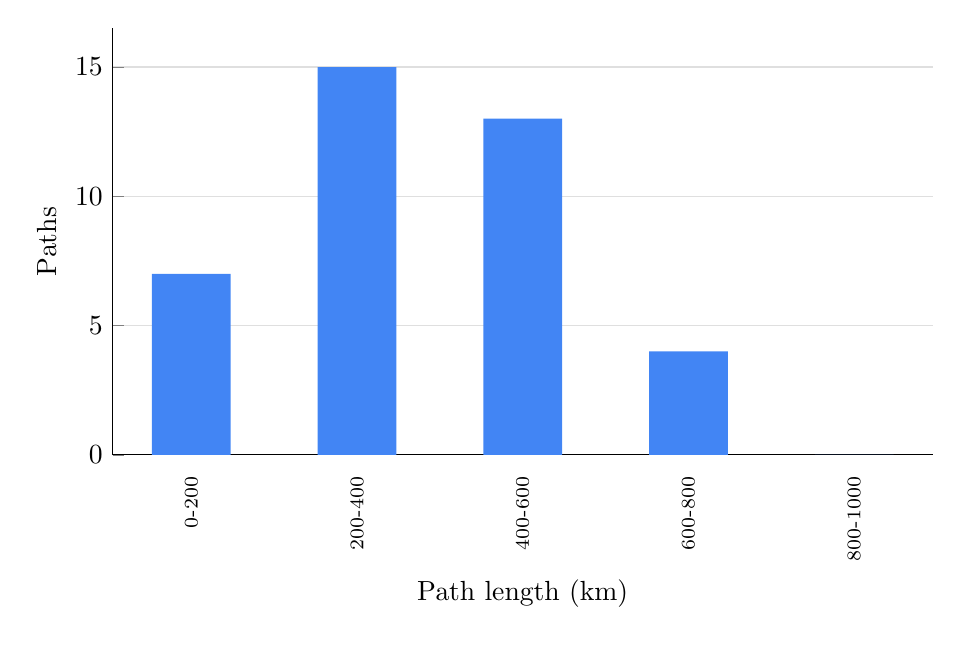
\begin{tikzpicture}
\begin{axis}[
  ybar, bar width=1.000cm, width=12.000cm, height=7cm,
  ymin=0, ymajorgrids, grid style={gray!25}, axis lines*=left,
  enlarge x limits={abs=1.000cm}, xtick=data, major x tick style={draw=none},
  x tick label style={rotate=90, font=\scriptsize, /pgf/number format/1000 sep=},
  legend style={at={(0.5,-0.3)}, anchor=north, legend columns=-1, draw=none},
  ylabel={Paths},
  xlabel={Path length (km)},
  symbolic x coords={0-200,200-400,400-600,600-800,800-1000,1000-1200,1200-1400,1400-1600,1600-1800,1800-2000}]
\addplot[fill={rgb,255:red,66;green,133;blue,244}, draw=none] coordinates {(0-200,7.000) (200-400,15.000) (400-600,13.000) (600-800,4.000) (800-1000,0.000) };
\end{axis}
\end{tikzpicture}\end{center}
\clearpage
\section*{Utilization Entropy}
\begin{center}\begin{adjustbox}{max width=\linewidth}
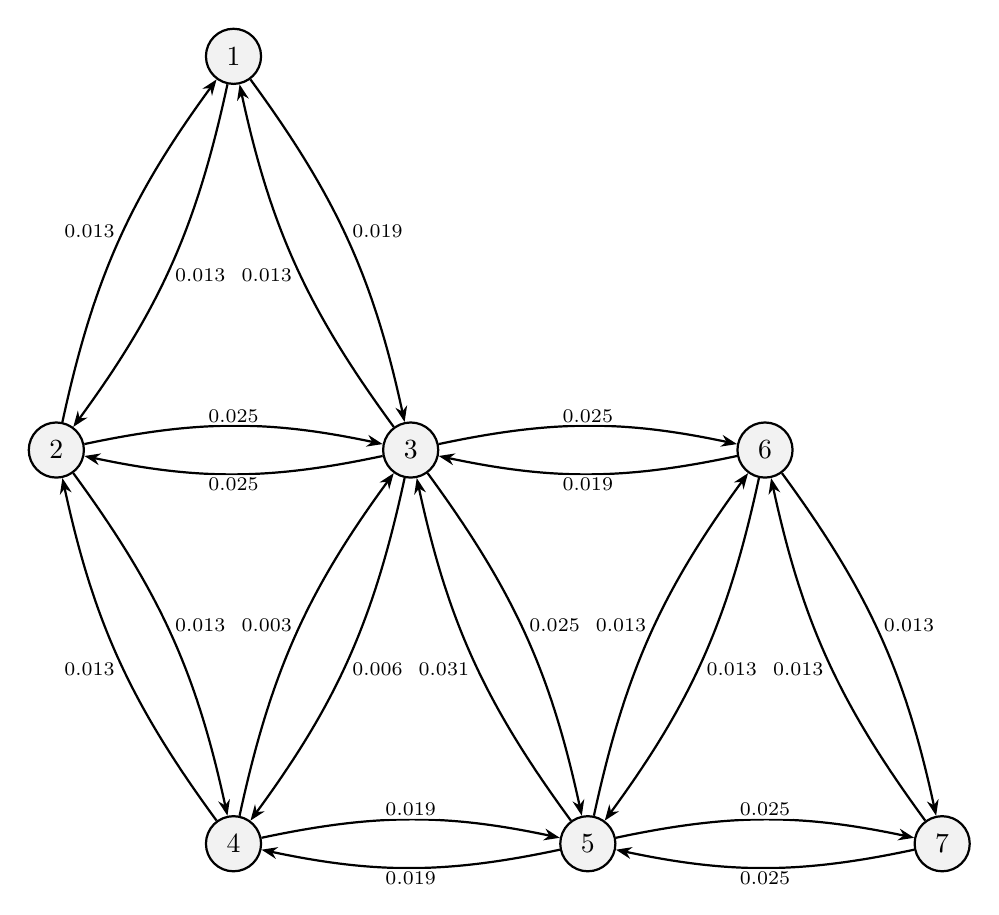
\begin{tikzpicture}[baseline, >={Stealth[length=2mm]},
  netnode/.style={circle, draw, thick, fill=gray!10, minimum size=7mm, inner sep=1pt},
  link/.style={thick},
  linklabel/.style={font=\scriptsize, inner sep=1pt, fill=white, fill opacity=0.85, text opacity=1}]
\node[netnode] (S1) at (2.250,10.000) {1};
\node[netnode] (S2) at (0.000,5.000) {2};
\node[netnode] (S3) at (4.500,5.000) {3};
\node[netnode] (S4) at (2.250,0.000) {4};
\node[netnode] (S5) at (6.750,0.000) {5};
\node[netnode] (S6) at (9.000,5.000) {6};
\node[netnode] (S7) at (11.250,0.000) {7};
\draw[link, ->] (S1) to[bend left=12] node[linklabel, auto] {0.013} (S2);
\draw[link, ->] (S1) to[bend left=12] node[linklabel, auto] {0.019} (S3);
\draw[link, ->] (S2) to[bend left=12] node[linklabel, auto] {0.013} (S1);
\draw[link, ->] (S2) to[bend left=12] node[linklabel, auto] {0.025} (S3);
\draw[link, ->] (S2) to[bend left=12] node[linklabel, auto] {0.013} (S4);
\draw[link, ->] (S3) to[bend left=12] node[linklabel, auto] {0.013} (S1);
\draw[link, ->] (S3) to[bend left=12] node[linklabel, auto] {0.025} (S2);
\draw[link, ->] (S3) to[bend left=12] node[linklabel, auto] {0.006} (S4);
\draw[link, ->] (S3) to[bend left=12] node[linklabel, auto] {0.025} (S5);
\draw[link, ->] (S3) to[bend left=12] node[linklabel, auto] {0.025} (S6);
\draw[link, ->] (S4) to[bend left=12] node[linklabel, auto] {0.013} (S2);
\draw[link, ->] (S4) to[bend left=12] node[linklabel, auto] {0.003} (S3);
\draw[link, ->] (S4) to[bend left=12] node[linklabel, auto] {0.019} (S5);
\draw[link, ->] (S5) to[bend left=12] node[linklabel, auto] {0.031} (S3);
\draw[link, ->] (S5) to[bend left=12] node[linklabel, auto] {0.019} (S4);
\draw[link, ->] (S5) to[bend left=12] node[linklabel, auto] {0.013} (S6);
\draw[link, ->] (S5) to[bend left=12] node[linklabel, auto] {0.025} (S7);
\draw[link, ->] (S6) to[bend left=12] node[linklabel, auto] {0.019} (S3);
\draw[link, ->] (S6) to[bend left=12] node[linklabel, auto] {0.013} (S5);
\draw[link, ->] (S6) to[bend left=12] node[linklabel, auto] {0.013} (S7);
\draw[link, ->] (S7) to[bend left=12] node[linklabel, auto] {0.025} (S5);
\draw[link, ->] (S7) to[bend left=12] node[linklabel, auto] {0.013} (S6);
\end{tikzpicture}
\end{adjustbox}\end{center}

\begin{center}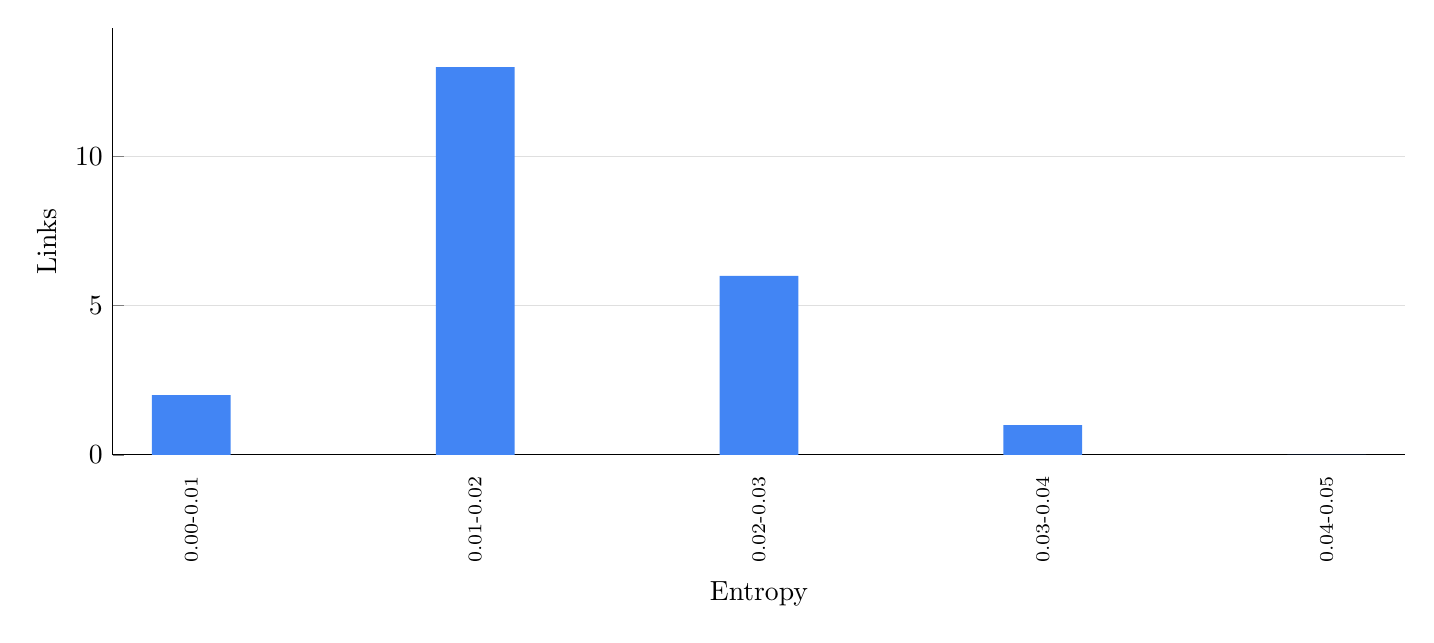
\begin{tikzpicture}
\begin{axis}[
  ybar, bar width=1.000cm, width=18.000cm, height=7cm,
  ymin=0, ymajorgrids, grid style={gray!25}, axis lines*=left,
  enlarge x limits={abs=1.000cm}, xtick=data, major x tick style={draw=none},
  x tick label style={rotate=90, font=\scriptsize, /pgf/number format/1000 sep=},
  legend style={at={(0.5,-0.3)}, anchor=north, legend columns=-1, draw=none},
  ylabel={Links},
  xlabel={Entropy},
  symbolic x coords={0.00-0.01,0.01-0.02,0.02-0.03,0.03-0.04,0.04-0.05,0.05-0.06,0.06-0.07,0.07-0.08,0.08-0.09,0.09-0.10,0.10-0.11,0.11-0.12,0.12-0.13,0.13-0.14,0.14-0.15,0.15-0.16,0.16-0.17,0.17-0.18,0.18-0.19,0.19-0.20,0.20-0.21,0.21-0.22,0.22-0.23,0.23-0.24,0.24-0.25,0.25-0.26,0.26-0.27,0.27-0.28,0.28-0.29,0.29-0.30,0.30-0.31,0.31-0.32,0.32-0.33,0.33-0.34,0.34-0.35,0.35-0.36,0.36-0.37,0.37-0.38,0.38-0.39,0.39-0.40,0.40-0.41,0.41-0.42,0.42-0.43,0.43-0.44,0.44-0.45,0.45-0.46,0.46-0.47,0.47-0.48,0.48-0.49,0.49-0.50,0.50-0.51,0.51-0.52,0.52-0.53,0.53-0.54,0.54-0.55,0.55-0.56,0.56-0.57,0.57-0.58,0.58-0.59,0.59-0.60,0.60-0.61,0.61-0.62,0.62-0.63,0.63-0.64,0.64-0.65,0.65-0.66,0.66-0.67,0.67-0.68,0.68-0.69,0.69-0.70,0.70-0.71,0.71-0.72,0.72-0.73,0.73-0.74,0.74-0.75,0.75-0.76,0.76-0.77,0.77-0.78,0.78-0.79,0.79-0.80,0.80-0.81,0.81-0.82,0.82-0.83,0.83-0.84,0.84-0.85,0.85-0.86,0.86-0.87,0.87-0.88,0.88-0.89,0.89-0.90,0.90-0.91,0.91-0.92,0.92-0.93,0.93-0.94,0.94-0.95,0.95-0.96,0.96-0.97,0.97-0.98,0.98-0.99,0.99-1.00}]
\addplot[fill={rgb,255:red,66;green,133;blue,244}, draw=none] coordinates {(0.00-0.01,2.000) (0.01-0.02,13.000) (0.02-0.03,6.000) (0.03-0.04,1.000) (0.04-0.05,0.000) };
\end{axis}
\end{tikzpicture}\end{center}
\clearpage
\section*{Shannon Entropy}
\begin{center}\begin{adjustbox}{max width=\linewidth}
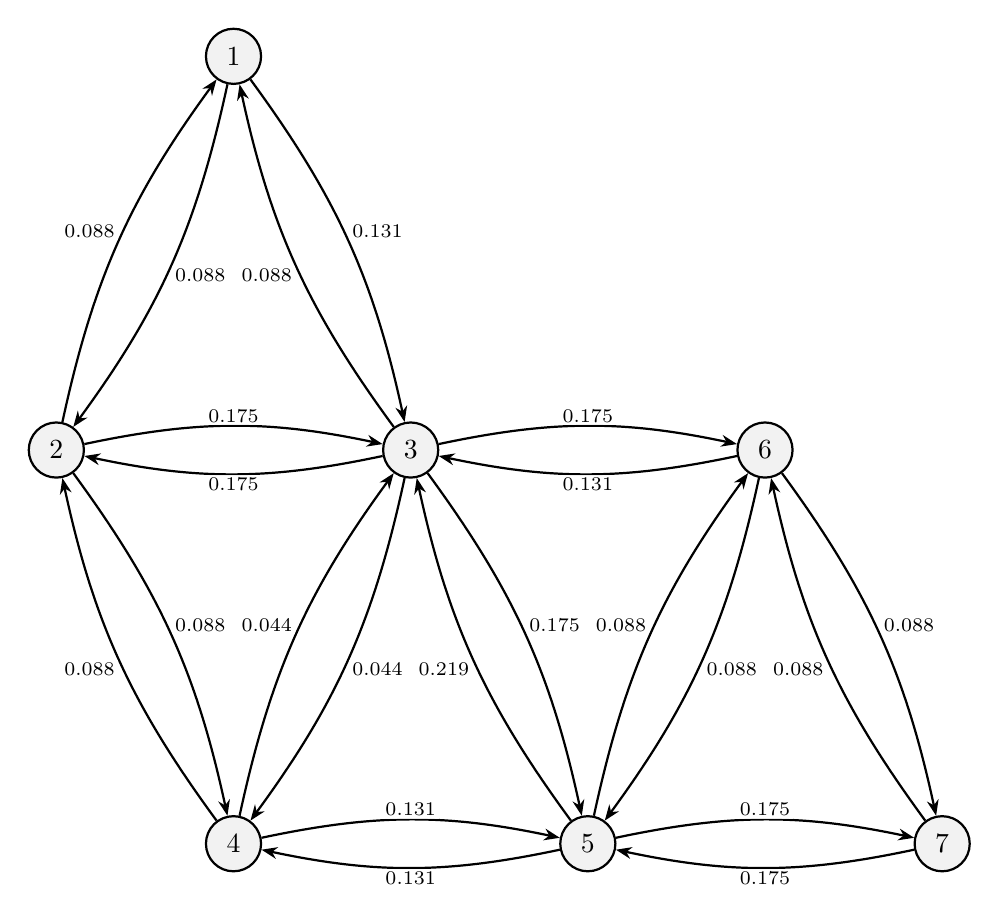
\begin{tikzpicture}[baseline, >={Stealth[length=2mm]},
  netnode/.style={circle, draw, thick, fill=gray!10, minimum size=7mm, inner sep=1pt},
  link/.style={thick},
  linklabel/.style={font=\scriptsize, inner sep=1pt, fill=white, fill opacity=0.85, text opacity=1}]
\node[netnode] (S1) at (2.250,10.000) {1};
\node[netnode] (S2) at (0.000,5.000) {2};
\node[netnode] (S3) at (4.500,5.000) {3};
\node[netnode] (S4) at (2.250,0.000) {4};
\node[netnode] (S5) at (6.750,0.000) {5};
\node[netnode] (S6) at (9.000,5.000) {6};
\node[netnode] (S7) at (11.250,0.000) {7};
\draw[link, ->] (S1) to[bend left=12] node[linklabel, auto] {0.088} (S2);
\draw[link, ->] (S1) to[bend left=12] node[linklabel, auto] {0.131} (S3);
\draw[link, ->] (S2) to[bend left=12] node[linklabel, auto] {0.088} (S1);
\draw[link, ->] (S2) to[bend left=12] node[linklabel, auto] {0.175} (S3);
\draw[link, ->] (S2) to[bend left=12] node[linklabel, auto] {0.088} (S4);
\draw[link, ->] (S3) to[bend left=12] node[linklabel, auto] {0.088} (S1);
\draw[link, ->] (S3) to[bend left=12] node[linklabel, auto] {0.175} (S2);
\draw[link, ->] (S3) to[bend left=12] node[linklabel, auto] {0.044} (S4);
\draw[link, ->] (S3) to[bend left=12] node[linklabel, auto] {0.175} (S5);
\draw[link, ->] (S3) to[bend left=12] node[linklabel, auto] {0.175} (S6);
\draw[link, ->] (S4) to[bend left=12] node[linklabel, auto] {0.088} (S2);
\draw[link, ->] (S4) to[bend left=12] node[linklabel, auto] {0.044} (S3);
\draw[link, ->] (S4) to[bend left=12] node[linklabel, auto] {0.131} (S5);
\draw[link, ->] (S5) to[bend left=12] node[linklabel, auto] {0.219} (S3);
\draw[link, ->] (S5) to[bend left=12] node[linklabel, auto] {0.131} (S4);
\draw[link, ->] (S5) to[bend left=12] node[linklabel, auto] {0.088} (S6);
\draw[link, ->] (S5) to[bend left=12] node[linklabel, auto] {0.175} (S7);
\draw[link, ->] (S6) to[bend left=12] node[linklabel, auto] {0.131} (S3);
\draw[link, ->] (S6) to[bend left=12] node[linklabel, auto] {0.088} (S5);
\draw[link, ->] (S6) to[bend left=12] node[linklabel, auto] {0.088} (S7);
\draw[link, ->] (S7) to[bend left=12] node[linklabel, auto] {0.175} (S5);
\draw[link, ->] (S7) to[bend left=12] node[linklabel, auto] {0.088} (S6);
\end{tikzpicture}
\end{adjustbox}\end{center}

\begin{center}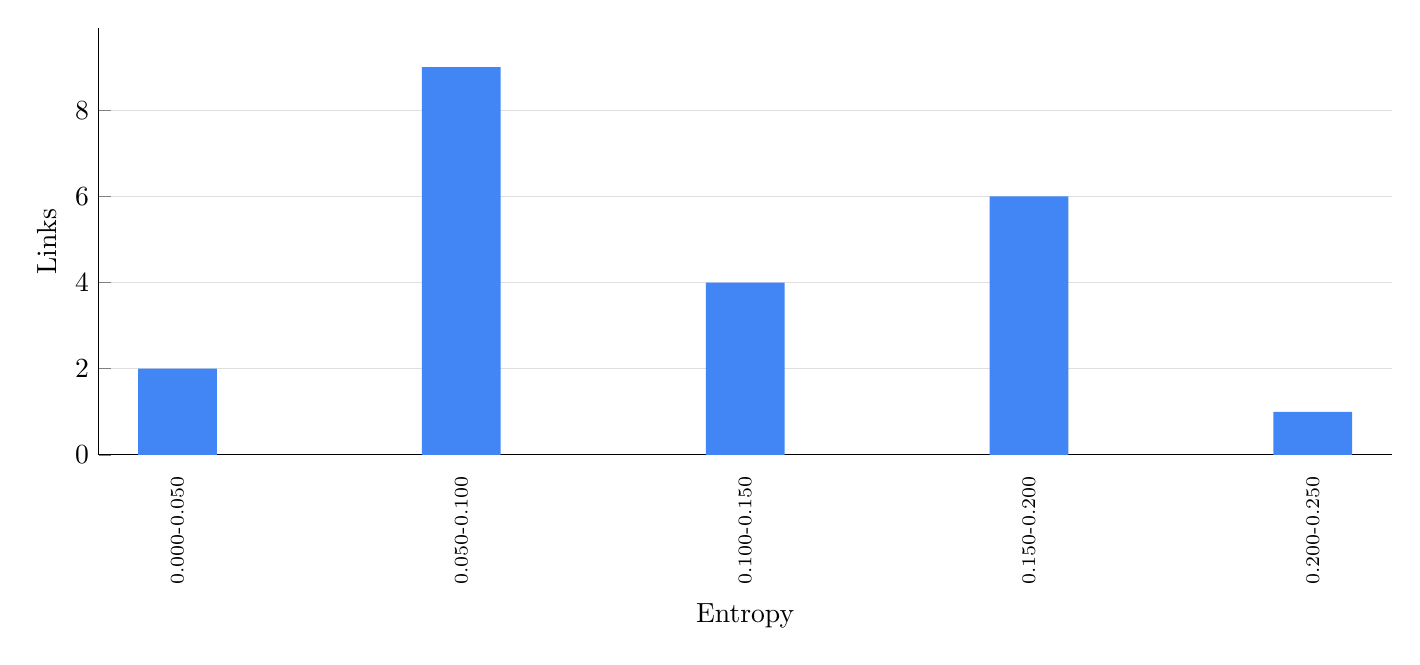
\begin{tikzpicture}
\begin{axis}[
  ybar, bar width=1.000cm, width=18.000cm, height=7cm,
  ymin=0, ymajorgrids, grid style={gray!25}, axis lines*=left,
  enlarge x limits={abs=1.000cm}, xtick=data, major x tick style={draw=none},
  x tick label style={rotate=90, font=\scriptsize, /pgf/number format/1000 sep=},
  legend style={at={(0.5,-0.3)}, anchor=north, legend columns=-1, draw=none},
  ylabel={Links},
  xlabel={Entropy},
  symbolic x coords={0.000-0.050,0.050-0.100,0.100-0.150,0.150-0.200,0.200-0.250,0.250-0.300,0.300-0.350,0.350-0.400,0.400-0.450,0.450-0.500,0.500-0.550,0.550-0.600,0.600-0.650,0.650-0.700,0.700-0.750,0.750-0.800,0.800-0.850,0.850-0.900,0.900-0.950,0.950-1.000}]
\addplot[fill={rgb,255:red,66;green,133;blue,244}, draw=none] coordinates {(0.000-0.050,2.000) (0.050-0.100,9.000) (0.100-0.150,4.000) (0.150-0.200,6.000) (0.200-0.250,1.000) };
\end{axis}
\end{tikzpicture}\end{center}

\end{document}
